\chapter{Das Automatisierungswerkzeuge für \LaTeX}
\label{automate}
Wenn in \LaTeX geschrieben wird kommt es sehr bald dazu, dass man für sein Dokument Referenzen(\verb|\cite{}|) bzw. ein Literaturverzeichnis benutzen möchte. Dafür gibt es verschiedene Bibliography Pakete unter anderem Biblatex mit dem Backend \emph{Biber}. Dies führt dazu, dass neben pdflatex ebenfalls noch biber aufgerufen werden muss. In \href{www.overleaf.com}{Overleaf} wird dies automatisch für den Nutzer getan. Für alle die jedoch auf ihrem eigenen Rechner, also lokal mit \LaTeX schreiben, bedeutet es mehrere Aufrufe durchführen zu müssen. Hierbei gibt es nun verschiedene Wege. Unter TexStudio zum Beispiel kann in den Optionen der Aufruf automatisiert werden. Dazu muss in den Build bzw. Erzeugen Einstellungen der Ablauf angepasst werden. Öffnet dazu Optionen > TexStudio Konfigurieren > Erzeugen > Standardcompiler Button um die Reihenfolge anzupassen. 
\begin{figure}[ht]
	\centering
	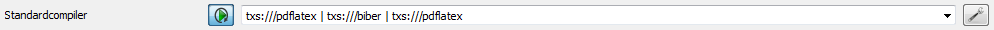
\includegraphics[width=\textwidth]{images/texstudio_option_build.PNG}
	\caption{Einstellungen für Biber in der Übersicht}
	\label{figbuild}
\end{figure}

In dem Optionsfenster \ref{figbuildOptions} kann dann die Option Biber und PdfLatex hinzugefügt werden. Für alle die kein TexStudio verwenden sondern über die Konsole ihre \LaTeX Dokumente compilieren gibt es die Automatisierungstools \emph{Arara} und \emph{LatexMK}. Diese beiden Werkzeuge werden ebenfalls häufig genutzt, wenn die Erstellung des Dokumentes sehr komplex wird und auch Dateien zwischendurch gelöscht werden müssen. Für dieses Template wurden die Optionen für \emph{Arara} bereits in die Preamble des Dokumentes hinzugefügt. Wie es benutzen ist erkläre ich im nächsten Abschnitt.

\begin{figure}[ht]
	\centering
	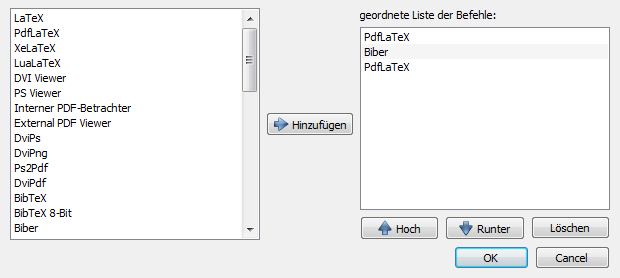
\includegraphics[width=\textwidth]{images/texstudio_optionwindow_build.PNG}
	\caption{Einstellungen für Biber im Optionsfenster}
	\label{figbuildOptions}
\end{figure}


\section{Arara}
arara ist ein TEX-Automatisierungswerkzeug, das auf Regeln und Richtlinien basiert. Es ist in mancher Hinsicht ähnlich wie andere bekannte Tools, wie z.B. latexmk\autocite{latexmk} und rubber\autocite{rubber}. Der Hauptunterschied ist die Tatsache, dass arara auf explizite Anweisungen im Quellcode nachschaut. Durch diese weiß arara was zu tun ist, anstatt sich auf andere Ressourcen, wie z.B. Logfile-Analyse oder MakeFiles zu verlassen. Der Link zum Gihtub Repository ist \url{https://github.com/cereda/arara}. 
%\url{https://texwelt.de/wissen/fragen/8764/was-ist-arara}

Wie schon beschrieben erkennt arara nicht von selbst was es tun soll und ist auf Anweisungen im Quelltext angewiesen. Diese können so aussehen:
\begin{lstlisting}[style=LaTeX]
% arara: pdflatex
% arara: biber
% arara: pdflatex
% arara: pdflatex
\end{lstlisting}

In der Preamble wurden folgende Anweisungen definiert:
\begin{lstlisting}[style=LaTeX]
% arara: pdflatex  { action: nonstopmode, shell: on }
% arara: pdflatex  { action: nonstopmode, shell: on }
% arara: biber
% arara: pdflatex  { action: nonstopmode, shell: on }
% arara: pdflatex  { action: nonstopmode, shell: on }
% arara: clean: { files: [ Index.aux, Index.bbl ] }
% arara: clean: { files: [ Index.bcf, Index.cod ] } 
% arara: clean: { files: [ Index.blg, Index.lof ] }
% arara: clean: { files: [ Index.lot, Index.out ] } 
% arara: clean: { files: [ Index.toc, Index.log ] } 
% arara: clean: { files: [ Index.run.xml ] }
\end{lstlisting}

Die Anweisungen definieren das pdflatex mit den Modi nonstopmode und --shell-escape ausgeführt werden soll. Nach pdflatex wird mit der Anweisung \emph{clean} und der Option \emph{files} noch überflüssigen Dateien entfernt. 
Die Installationsbeschreibung für Windows im Handbuch von arara ist etwas verwirrend, weswegen hier die Installation-Schritte beschrieben werden:
\begin{enumerate}
\item Miktex Update Manager(Admin) starten und aktualisieren lassen
\item Miktex Package Manager starten und dort nachdem Paket arara suchen
\item Paket installieren. (Nutzt nicht in der packages.tex \verb|\usepackage{arara}|)	
\end{enumerate}

Wenn man dann arara noch in TexStudio integrieren möchte sollte man diesen Link aufrufen und lesen. Es funktioniert ähnlich wie, zum Beginn des Kapitels beschrieben, für Biber, nur das man seinen eigenen Prozess definiert. Dazu muss man den Pfad zur Exe kopieren und wie in dem Thread beschrieben wird TexStudio hinzufügen.

Hier der Link: \url{https://tex.stackexchange.com/questions/313616/configuring-arara-in-texstudio-on-windows}

Wenn der Standardcompiler dann auf arara gesetzt wurde drückt man wie gewohnt F5 oder auf den Compiler-Button(Grüner Pfeil).
Für alle die Plots erstellen möchten, ist dies hier ebenfalls interessant: \url{https://latex.org/know-how/435-gnuplot-arara}
Wer Hilfe benötigt beim Einstellen von arara kann auch auf Gitter.im vorbeischauen. Dort gibt es einen Channel indem aktiv geholfen wird. 
\section{LatexMK}
Wie bereits beschrieben reiht sich LatexMK als Automatisierungstool in die Reihe der nützlichen Tools ein. Die Installation von LatexMK erfolgt dabei ebenfalls über den Paket Manager von Miktex oder bei Linux über texlive. Die Handhabung ist hierbei jedoch eine ganz andere als bei \emph{arara}, da dieses Tool keine Anweisungen benötigt. Es kann ebenfalls als Standardcompiler in TexStudio über die bereits beschriebene Methodik festgelegt und kann ebenfalls über die Shell gestartet werden. Hier ein Beispiel: 

\begin{lstlisting}[style=Bash]
$ latexmk -pdf -pv myfile.tex
\end{lstlisting}

Der Vorteil von LatexMK ist, dass es automatisch erkennen kann ob eine Datei verändert wurde. Über die Option \emph{-pv} wird dem Tool mitgeteilt, dass es jedes mal kompilieren soll wenn die Datei verändert wurde. Weitere Erklärungen und Anleitungen findet man hier:
\begin{description}
	\item[Dokumentation: ] \url{http://mg.readthedocs.io/latexmk.html}
	\item[Hauptseite von LatexMK: ] \url{http://personal.psu.edu/jcc8//latexmk/}
	\item[Handbuch des Paketes: ] \url{http://ftp.uni-erlangen.de/ctan/support/latexmk/latexmk.pdf}
\end{description}

\section{Rubber}
Rubber ist ein Programm, dessen Zweck es ist, alle Aufgaben im Zusammenhang mit der Erstellung von LaTeX-Dokumenten zu erledigen. Dazu gehört natürlich auch, das Dokument selbst so oft zu kompilieren, dass alle Referenzen definiert sind. Zur Verwaltung der bibliographischen Referenzen wird BibTeX verwendet. Die automatische Ausführung von dvips zur Erzeugung von PostScript-Dokumenten ist ebenso enthalten wie die Verwendung von pdfLaTeX zur Erzeugung von PDF-Dokumenten. Die Quellenseite von \emph{rubber} ist: \url{https://launchpad.net/rubber} . Das Programm funktioniert wie LatexMK und muss entweder über die Shell genutzt oder wie \emph{arara} in TexStudio als User Command eingebunden werden. Der Aufruf ist ähnlich wie in LatexMK: 

\begin{lstlisting}[style=Bash]
$ rubber --clean --pdf myfile
\end{lstlisting}

In diesem Blog-Eintrag auf Tex-talk.net erklärt der Erfinder von \emph{arara} wie rubber funktioniert: \url{http://tex-talk.net/2011/12/building-documents-with-rubber/} .
